\FloatBarrier

% Problema \getNumeroProblema (Basato su Kharef P3)
\begin{table}[htbp]
  \centering
  \renewcommand{\arraystretch}{1.5}
  \begin{tabular}{|>{\raggedright\arraybackslash}p{7.5cm}|>{\raggedright\arraybackslash}p{7.5cm}|}
    \hline
    \rowcolor{green!30}
    \multicolumn{2}{|c|}{\textbf{Problema \getNumeroProblema}} \\
    \hline
    \textbf{Descrizione} & La funzionalità di ricerca nella pagina "Esplora Appunti" è limitata al solo titolo del documento. \\
    \hline
    \textbf{Pagina del sito} & Esplora Appunti \\
    \hline
    \textbf{Principi violati} & 6 (Flessibilità ed efficienza d'uso) \\
    \hline
    \textbf{Grado di severità} & 3 (Problema rilevante)  \\
    \hline
    \textbf{Nome del valutatore} & Kharef  \\
    \hline
  \end{tabular}
\end{table}

% Problema \getNumeroProblema (Basato su Kharef P4)
\begin{table}[htbp]
  \centering
  \renewcommand{\arraystretch}{1.5}
  \begin{tabular}{|>{\raggedright\arraybackslash}p{7.5cm}|>{\raggedright\arraybackslash}p{7.5cm}|}
    \hline
    \rowcolor{green!30}
    \multicolumn{2}{|c|}{\textbf{Problema \getNumeroProblema}} \\
    \hline
    \textbf{Descrizione} & L'azione di caricare un nuovo documento è accessibile solo dalla pagina "I Miei Appunti". Non è presente un pulsante di accesso rapido ("Carica" o "+") nella barra di navigazione principale o nella dashboard. \\
    \hline
    \textbf{Pagina del sito} & Dashboard \\
    \hline
    \textbf{Principi violati} & 4 (Assicurare consistenza); 6 (Assicurare flessibilità ed efficienza d’uso) \\
    \hline
    \textbf{Grado di severità} & 2 (Problema secondario)  \\
    \hline
    \textbf{Screen} &
    \vspace{10pt}
    \hspace*{\fill}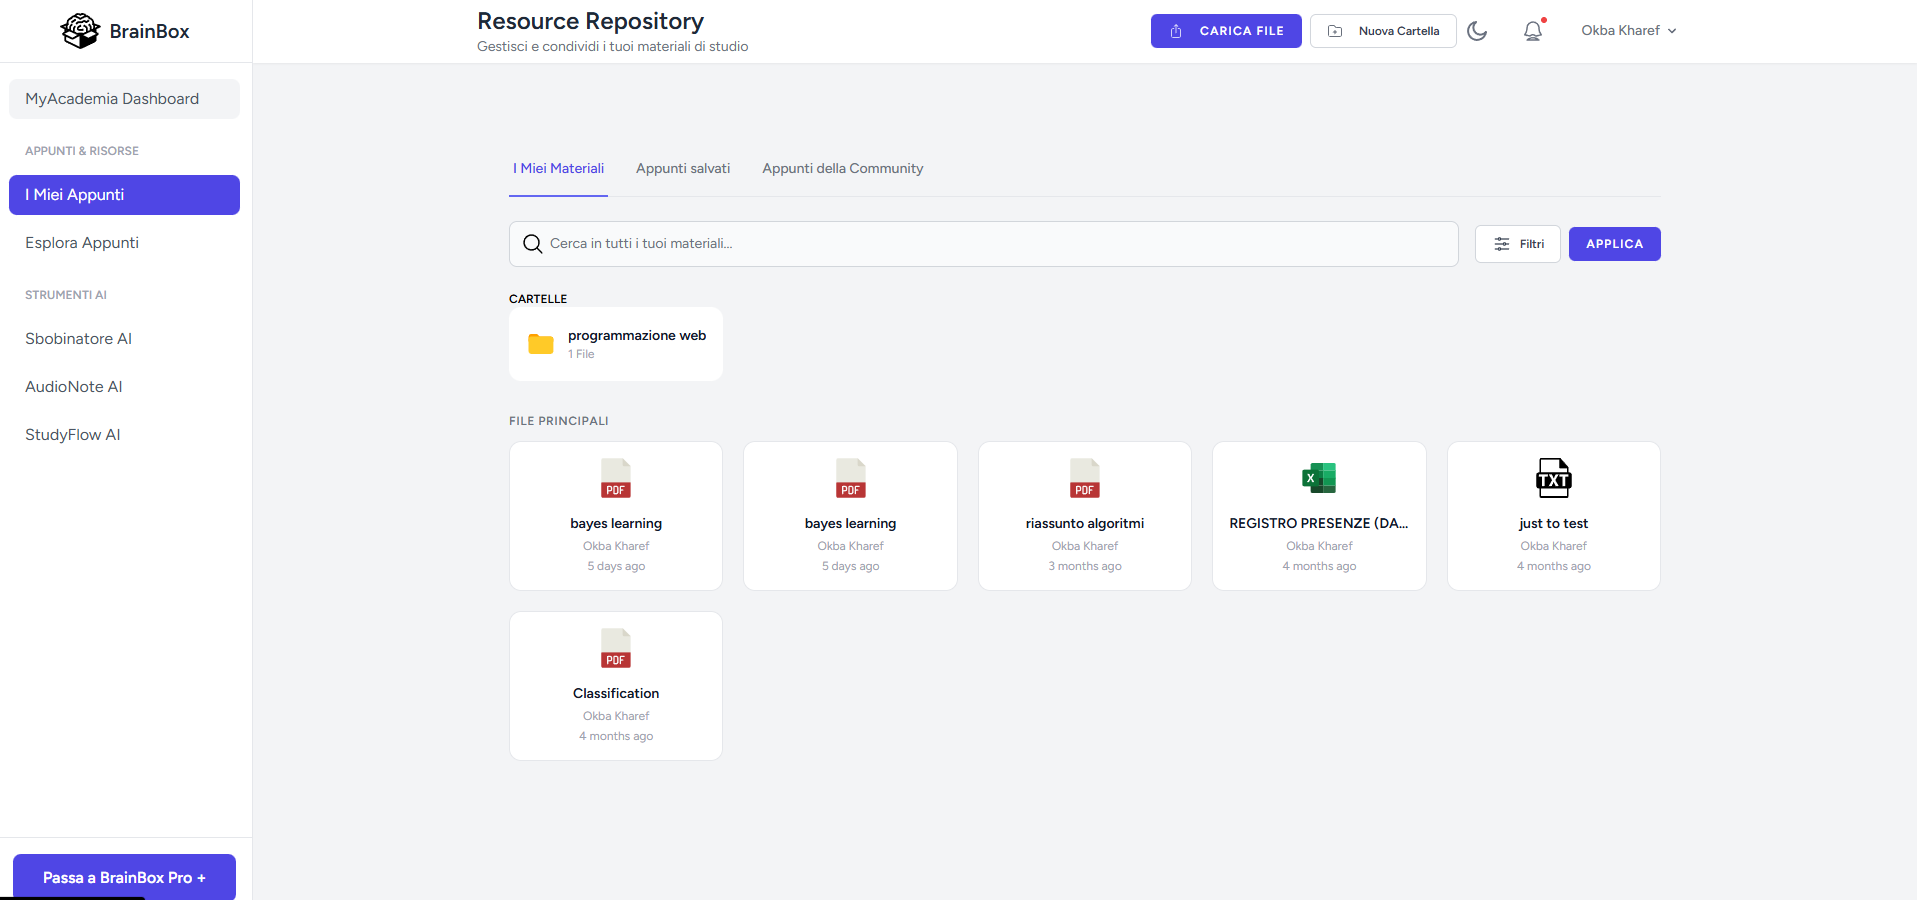
\includegraphics[width=6.5cm]{Screenshots/foglio3/problema62.png}\hspace*{\fill}
    \vspace{10pt}
    \\
    \hline
    \textbf{Nome del valutatore} & Kharef \\
    \hline
  \end{tabular}
\end{table}

% Problema \getNumeroProblema (Basato su Kharef P6)
\begin{table}[htbp]
  \centering
  \renewcommand{\arraystretch}{1.5}
  \begin{tabular}{|>{\raggedright\arraybackslash}p{7.5cm}|>{\raggedright\arraybackslash}p{7.5cm}|}
    \hline
    \rowcolor{green!30}
    \multicolumn{2}{|c|}{\textbf{Problema \getNumeroProblema}} \\
    \hline
    \textbf{Descrizione} & Il processo di registrazione in due fasi non fornisce indicatori di progresso (es. "Passo 1 di 2"). L'utente non sa che ci sarà un secondo passaggio, il che rende l'apparizione del secondo form inaspettata. \\
    \hline
    \textbf{Pagina del sito} & Registrazione \\
    \hline
    \textbf{Principi violati} & 1 (Visibilità dello stato del sistema); 3 (Controllo dell’utente e libertà) \\
    \hline
    \textbf{Grado di severità} & 3 (Problema rilevante) \\
    \hline
    \textbf{Screen} &
    \vspace{10pt}
    \hspace*{\fill}
    \begin{minipage}{0.48\linewidth}
      \centering
      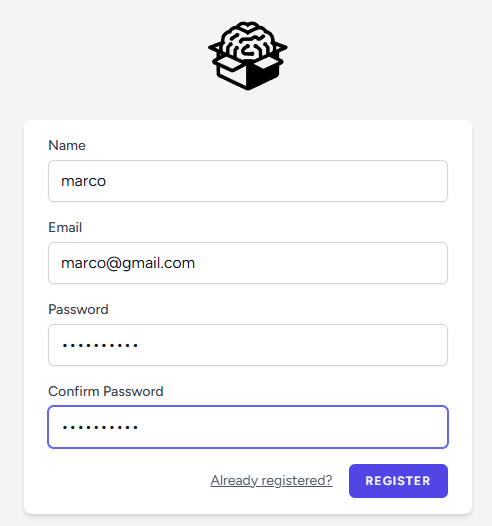
\includegraphics[width=3.5cm]{Screenshots/foglio3/problema64a.png}
    \end{minipage}
    \hfill
    \begin{minipage}{0.48\linewidth}
      \centering
      
\includegraphics[width=3.5cm]{Screenshots/foglio3/problema64b.png}
    \end{minipage}
    \hspace*{\fill}
    \vspace{10pt}
    \\
    \hline
    \textbf{Nome del valutatore} & Kharef \\
    \hline
  \end{tabular}
\end{table}

% Problema \getNumeroProblema (Basato su Kharef P7)
\begin{table}[htbp]
  \centering
  \renewcommand{\arraystretch}{1.5}
  \begin{tabular}{|>{\raggedright\arraybackslash}p{7.5cm}|>{\raggedright\arraybackslash}p{7.5cm}|}
    \hline
    \rowcolor{green!30}
    \multicolumn{2}{|c|}{\textbf{Problema \getNumeroProblema}} \\
    \hline
    \textbf{Descrizione} & Manca consistenza nella terminologia delle azioni. Nella pagina "I Miei Appunti", l'azione primaria si chiama "Scarica", ma all'interno della pagina dettaglio si chiama "download". \\
    \hline
    \textbf{Pagina del sito} & I Miei Appunti \\
    \hline
    \textbf{Principi violati} & 2 (Adeguare il sistema al mondo reale); 4 (Assicurare consistenza)  \\
    \hline
    \textbf{Grado di severità} & 2 (Problema secondario)  \\
    \hline
    \textbf{Screen} &
    \vspace{10pt}
    \hspace*{\fill}
    \begin{minipage}{0.48\linewidth}
      \centering
      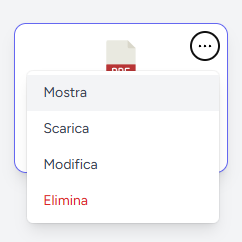
\includegraphics[width=3.5cm]{Screenshots/foglio3/problema65a.png}
    \end{minipage}
    \hfill
    \begin{minipage}{0.48\linewidth}
      \centering
      
\includegraphics[width=3.5cm]{Screenshots/foglio3/problema65b.png}
    \end{minipage}
    \hspace*{\fill}
    \vspace{10pt}
    \\
    \hline
    \textbf{Nome del valutatore} & Kharef \\
    \hline
  \end{tabular}
\end{table}

% Problema \getNumeroProblema (Basato su Kharef P10)
\begin{table}[htbp]
  \centering
  \renewcommand{\arraystretch}{1.5}
  \begin{tabular}{|>{\raggedright\arraybackslash}p{7.5cm}|>{\raggedright\arraybackslash}p{7.5cm}|}
    \hline
    \rowcolor{green!30}
    \multicolumn{2}{|c|}{\textbf{Problema \getNumeroProblema}} \\
    \hline
    \textbf{Descrizione} & Dopo aver caricato con successo un nuovo appunto, l'utente viene reindirizzato alla lista "I Miei Appunti", ma non c'è nessuna indicazione visiva (es. un'evidenziazione temporanea) che indichi quale sia il nuovo elemento appena aggiunto. \\
    \hline
    \textbf{Pagina del sito} & I Miei Appunti \\
    \hline
    \textbf{Principi violati} & 1 (Far vedere lo stato del sistema)\\
    \hline
    \textbf{Grado di severità} & 1 (Problema accessorio) \\
    \hline
    \textbf{Screen} &
    \vspace{10pt}
    \hspace*{\fill}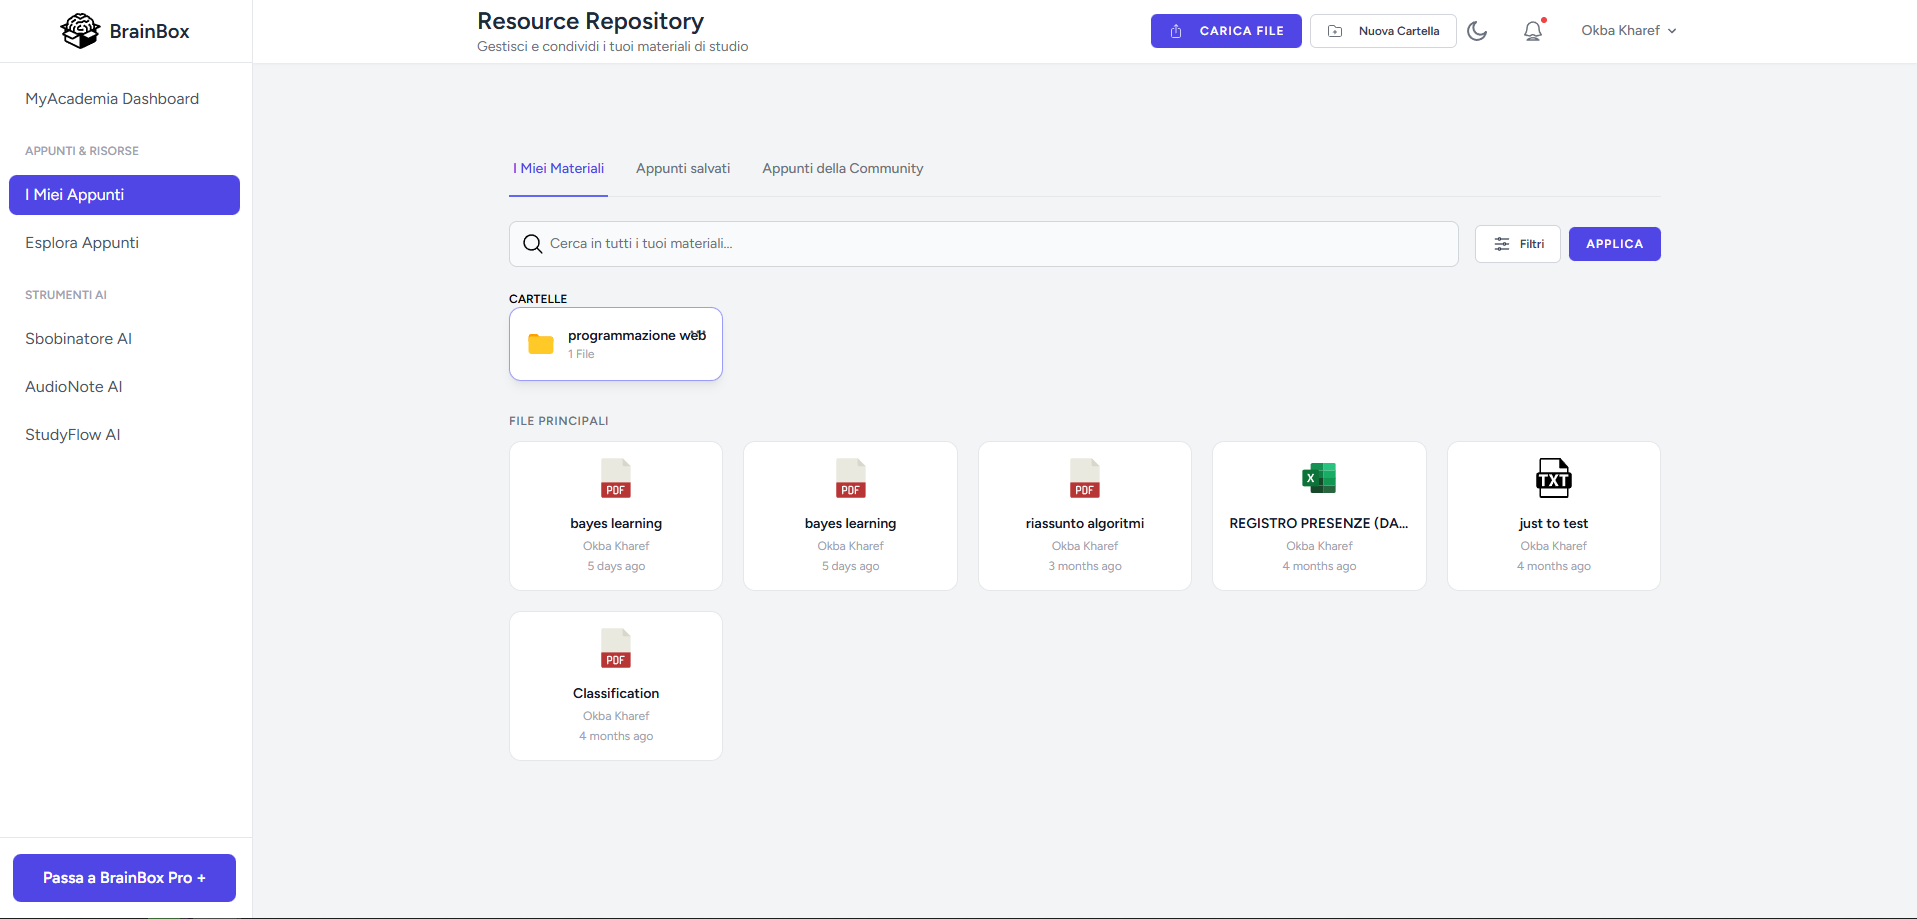
\includegraphics[width=6.5cm]{Screenshots/foglio3/problema68.png}\hspace*{\fill}
    \vspace{10pt}
    \\
    \hline
    \textbf{Nome del valutatore} & Kharef \\
    \hline
  \end{tabular}
\end{table}

% Problema \getNumeroProblema (Basato su Kharef P11)
\begin{table}[htbp]
  \centering
  \renewcommand{\arraystretch}{1.5}
  \begin{tabular}{|>{\raggedright\arraybackslash}p{7.5cm}|>{\raggedright\arraybackslash}p{7.5cm}|}
    \hline
    \rowcolor{green!30}
    \multicolumn{2}{|c|}{\textbf{Problema \getNumeroProblema}} \\
    \hline
    \textbf{Descrizione} & L'utente non ha alcun controllo sull'ordinamento delle liste di documenti (né in "I Miei Appunti" né in "Esplora Appunti"). I risultati sono presentati in un ordine predefinito senza opzioni di ordinamento (es. per popolarità, titolo, autore). \\
    \hline
    \textbf{Pagina del sito} & I Miei Appunti / Esplora Appunti \\
    \hline
    \textbf{Principi violati} & 3 (Controllo dell’utente e libertà); 6 (Assicurare flessibilità ed efficienza d’uso) \\
    \hline
    \textbf{Grado di severità} & 2 (Problema secondario) \\
    \hline
    \textbf{Screen} &
    \vspace{10pt}
    \hspace*{\fill}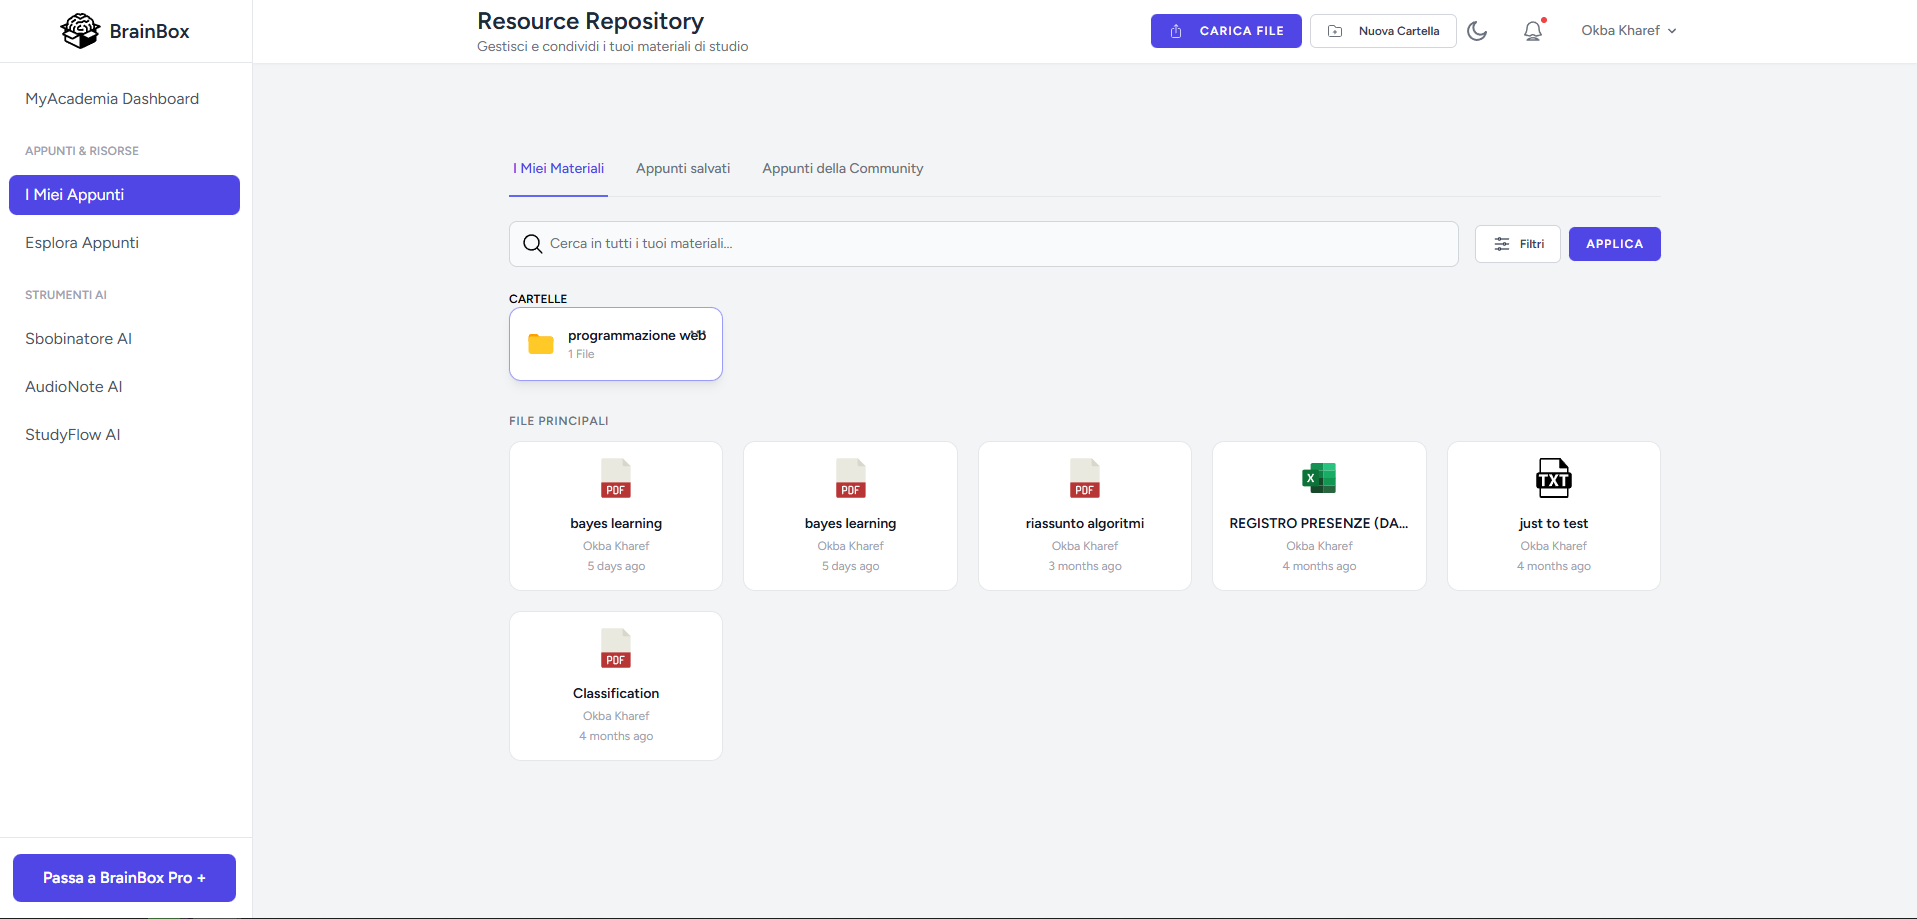
\includegraphics[width=6.5cm]{Screenshots/foglio3/problema68.png}\hspace*{\fill}
    \vspace{10pt}
    \\
    \hline
    \textbf{Nome del valutatore} & Kharef \\
    \hline
  \end{tabular}
\end{table}

% Problema \getNumeroProblema (Basato su Kharef P13)
\begin{table}[htbp]
  \centering
  \renewcommand{\arraystretch}{1.5}
  \begin{tabular}{|>{\raggedright\arraybackslash}p{7.5cm}|>{\raggedright\arraybackslash}p{7.5cm}|}
    \hline
    \rowcolor{green!30}
    \multicolumn{2}{|c|}{\textbf{Problema \getNumeroProblema}} \\
    \hline
    \textbf{Descrizione} & I messaggi di errore di validazione nei form, pur essendo presenti (es. Pagina "Sbobinatore AI"), sono generici e non sempre offrono una guida utile (es. "Il file non è valido" invece di "Il file supera la dimensione massima consentita"). \\
    \hline
    \textbf{Pagina del sito} & Area Utente \\
    \hline
    \textbf{Principi violati} & 1 (Far vedere lo stato del sistema); 9 (Permettere all’utente di correggere gli errori e non solo di rilevarli) \\
    \hline
    \textbf{Grado di severità} & 2 (Problema secondario) \\
    \hline
    \textbf{Nome del valutatore} & Kharef \\
    \hline
  \end{tabular}
\end{table}

% Problema \getNumeroProblema (Basato su Kharef P14)
\begin{table}[htbp]
  \centering
  \renewcommand{\arraystretch}{1.5}
  \begin{tabular}{|>{\raggedright\arraybackslash}p{7.5cm}|>{\raggedright\arraybackslash}p{7.5cm}|}
    \hline
    \rowcolor{green!30}
    \multicolumn{2}{|c|}{\textbf{Problema \getNumeroProblema}} \\
    \hline
    \textbf{Descrizione} & I messaggi di errore di validazione nei form non sono presenti se si tenta di caricare un file multimediale non supportato (ad esempio, nella Pagina "Sbobinatore AI"). \\
    \hline
    \textbf{Pagina del sito} & Area Utente \\
    \hline
    \textbf{Principi violati} & 1 (Far vedere lo stato del sistema); 9 (Permettere all’utente di correggere gli errori e non solo di rilevarli) \\
    \hline
    \textbf{Grado di severità} & 3 (Problema rilevante) \\
    \hline
    \textbf{Screen} &
    \vspace{10pt}
    \hspace*{\fill}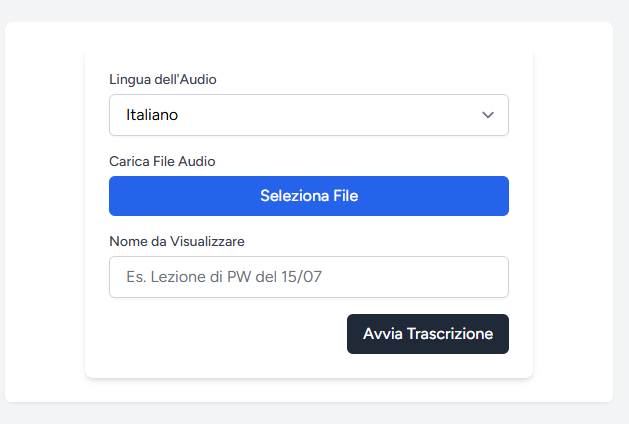
\includegraphics[width=6.5cm]{Screenshots/foglio3/problema72.png}\hspace*{\fill}
    \vspace{10pt}
    \\
    \hline
    \textbf{Nome del valutatore} & Kharef \\
    \hline
  \end{tabular}
\end{table}

% Problema \getNumeroProblema (Basato su Kharef P15)
\begin{table}[htbp]
  \centering
  \renewcommand{\arraystretch}{1.5}
  \begin{tabular}{|>{\raggedright\arraybackslash}p{7.5cm}|>{\raggedright\arraybackslash}p{7.5cm}|}
    \hline
    \rowcolor{green!30}
    \multicolumn{2}{|c|}{\textbf{Problema \getNumeroProblema}} \\
    \hline
    \textbf{Descrizione} & Nella pagina di dettaglio di un documento, non c'è una chiara separazione gerarchica tra i metadati del documento e la sezione dei commenti. Sono presentati come blocchi sequenziali di uguale importanza visiva. \\
    \hline
    \textbf{Pagina del sito} & I Miei Appunti - Visualizzazione Documento \\
    \hline
    \textbf{Principi violati} & 7 (Visualizzare tutte e sole le informazioni necessarie) \\
    \hline
    \textbf{Grado di severità} & 1 (Problema accessorio) \\
    \hline
    \textbf{Screen} &
    \vspace{10pt}
    \hspace*{\fill}
\includegraphics[height=6cm, keepaspectratio]{Screenshots/foglio3/problema73.png}\hspace*{\fill}
    \vspace{10pt}
    \\
    \hline
    \textbf{Nome del valutatore} & Kharef \\
    \hline
  \end{tabular}
\end{table}

% Problema \getNumeroProblema (Basato su Kharef P16)
\begin{table}[htbp]
  \centering
  \renewcommand{\arraystretch}{1.5}
  \begin{tabular}{|>{\raggedright\arraybackslash}p{7.5cm}|>{\raggedright\arraybackslash}p{7.5cm}|}
    \hline
    \rowcolor{green!30}
    \multicolumn{2}{|c|}{\textbf{Problema \getNumeroProblema}} \\
    \hline
    \textbf{Descrizione} & Non esiste un feedback visivo che distingua i link interni già visitati da quelli non ancora visitati, costringendo l'utente a ricordare quali contenuti ha già consultato. \\
    \hline
    \textbf{Pagina del sito} & I Miei Appunti / Esplora Appunti \\
    \hline
    \textbf{Principi violati} & 1 (Far vedere lo stato del sistema); 5 (Riconoscimento anziché ricordo) \\
    \hline
    \textbf{Grado di severità} & 1 (Problema accessorio) \\
    \hline
    \textbf{Screen} &
    \vspace{10pt}
    \hspace*{\fill}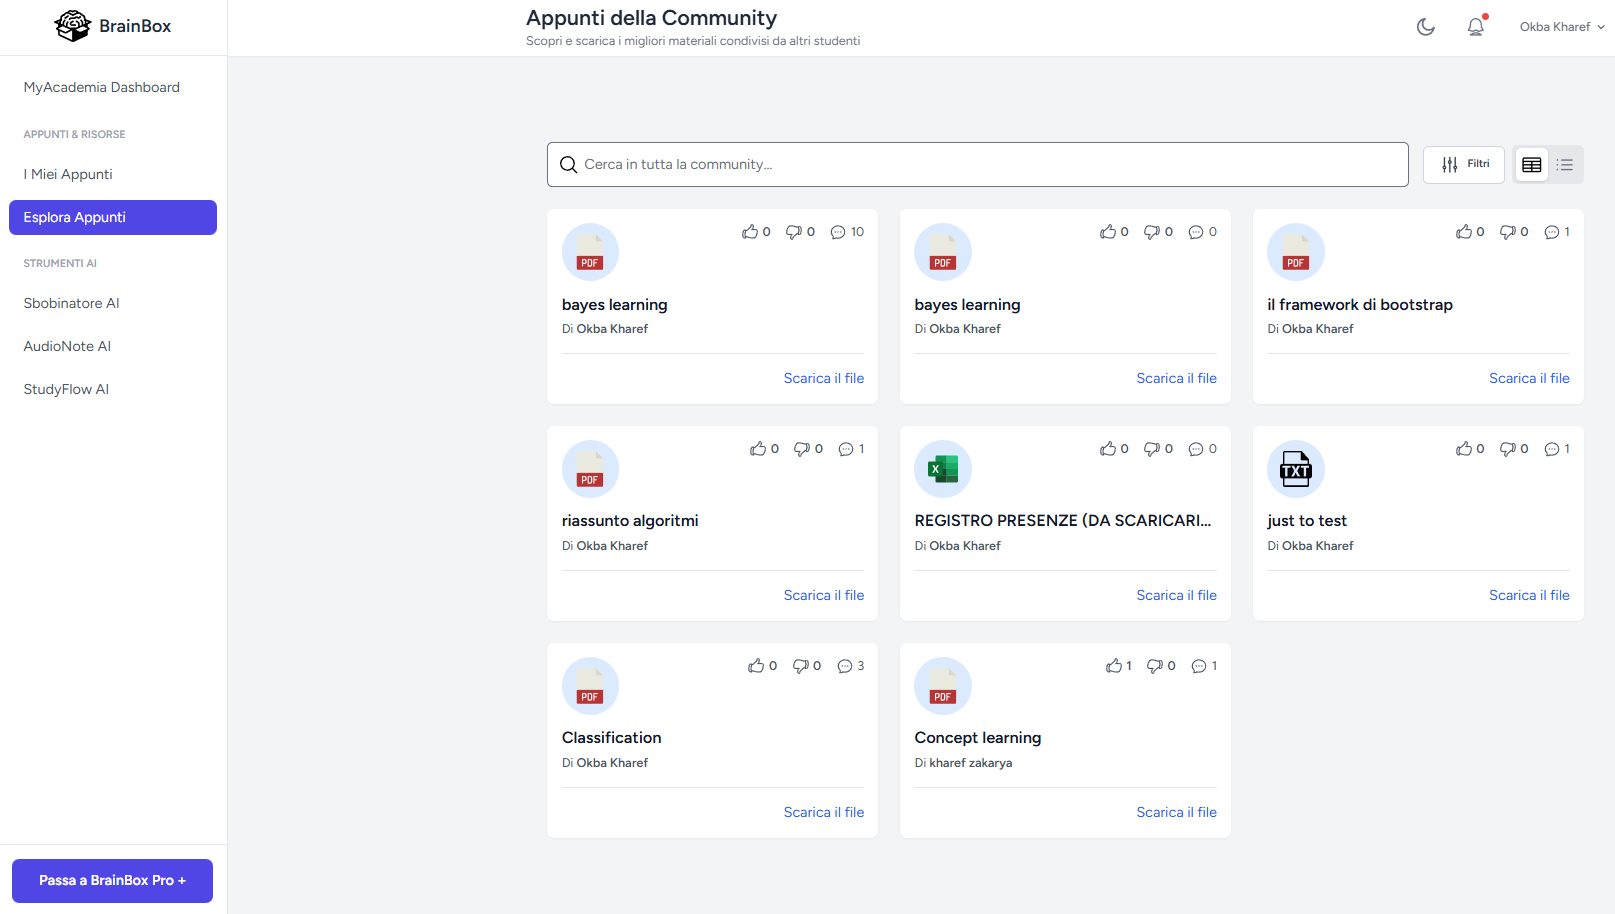
\includegraphics[width=6.5cm]{Screenshots/foglio3/problema74.png}\hspace*{\fill}
    \vspace{10pt}
    \\
    \hline
    \textbf{Nome del valutatore} & Kharef \\
    \hline
  \end{tabular}
\end{table}

% Problema \getNumeroProblema (Basato su Kharef P17)
\begin{table}[htbp]
  \centering
  \renewcommand{\arraystretch}{1.5}
  \begin{tabular}{|>{\raggedright\arraybackslash}p{7.5cm}|>{\raggedright\arraybackslash}p{7.5cm}|}
    \hline
    \rowcolor{green!30}
    \multicolumn{2}{|c|}{\textbf{Problema \getNumeroProblema}} \\
    \hline
    \textbf{Descrizione} & Non c'è modo per un utente di segnalare un commento o un documento inappropriato (es. offensivo, spam, violazione di copyright). \\
    \hline
    \textbf{Pagina del sito} & I Miei Appunti - Visualizzazione Documento \\
    \hline
    \textbf{Principi violati} & 3 (Controllo dell’utente e libertà) \\
    \hline
    \textbf{Grado di severità} & 2 (Problema rilevante) \\
    \hline
    \textbf{Nome del valutatore} & Kharef \\
    \hline
  \end{tabular}
\end{table}

% Problema \getNumeroProblema (Basato su Kharef P18)
\begin{table}[htbp]
  \centering
  \renewcommand{\arraystretch}{1.5}
  \begin{tabular}{|>{\raggedright\arraybackslash}p{7.5cm}|>{\raggedright\arraybackslash}p{7.5cm}|}
    \hline
    \rowcolor{green!30}
    \multicolumn{2}{|c|}{\textbf{Problema \getNumeroProblema}} \\
    \hline
    \textbf{Descrizione} & Il sistema non offre alcuna forma di salvataggio automatico o bozza. Il lavoro (descrizioni lunghe o commenti complessi) può essere perso in caso di caduta della connessione o chiusura accidentale della pagina. \\
    \hline
    \textbf{Pagina del sito} & I Miei Appunti \\
    \hline
    \textbf{Principi violati} & 8 (Prevenire gli errori) \\
    \hline
    \textbf{Grado di severità} & 3 (Problema rilevante)  \\
    \hline
    \textbf{Nome del valutatore} & Kharef \\
    \hline
  \end{tabular}
\end{table}

% Problema \getNumeroProblema (Basato su Kharef P20)
\begin{table}[htbp]
  \centering
  \renewcommand{\arraystretch}{1.5}
  \begin{tabular}{|>{\raggedright\arraybackslash}p{7.5cm}|>{\raggedright\arraybackslash}p{7.5cm}|}
    \hline
    \rowcolor{green!30}
    \multicolumn{2}{|c|}{\textbf{Problema \getNumeroProblema}} \\
    \hline
    \textbf{Descrizione} & I titoli dei file scaricati non sono formattati, il file scaricato ha un nome casuale (es. aGDvnS4viFvc9VSHFJDdA5dE6HvmkjshP hkiVCBV.pdf) invece di usare un nome descrittivo basato sul titolo del documento (es. Riassunto\_Analisi\_1-BrainBox.pdf). \\
    \hline
    \textbf{Pagina del sito} & Area Utente \\
    \hline
    \textbf{Principi violati} & 2 (Adeguare il sistema al mondo reale); 7 (Visualizzare tutte e sole le informazioni necessarie) \\
    \hline
    \textbf{Grado di severità} & 2 (Problema secondario) \\
    \hline
    \textbf{Screen} &
    \vspace{10pt}
    \hspace*{\fill}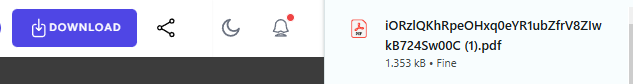
\includegraphics[width=6.5cm]{Screenshots/foglio3/problema78.png}\hspace*{\fill}
    \vspace{10pt}
    \\
    \hline
    \textbf{Nome del valutatore} & Kharef \\
    \hline
  \end{tabular}
\end{table}

% Problema \getNumeroProblema (Basato su Kharef P22)
\begin{table}[htbp]
  \centering
  \renewcommand{\arraystretch}{1.5}
  \begin{tabular}{|>{\raggedright\arraybackslash}p{7.5cm}|>{\raggedright\arraybackslash}p{7.5cm}|}
    \hline
    \rowcolor{green!30}
    \multicolumn{2}{|c|}{\textbf{Problema \getNumeroProblema}} \\
    \hline
    \textbf{Descrizione} & Su schermi di dispositivi mobili, la modifica dei commenti causa problemi di visualizzazione. Quando si modifica un commento, la pagina si riorganizza in modo confuso, gli elementi si spostano e la barra laterale non si adatta correttamente. \\
    \hline
    \textbf{Pagina del sito} & I Miei Appunti - Visualizzazione Documento \\
    \hline
    \textbf{Principi violati} & 3 (Controllo dell’utente e libertà); 7 (Visualizzare tutte e sole le informazioni necessarie) \\
    \hline
    \textbf{Grado di severità} & 2 (Problema secondario) \\
    \hline
    \textbf{Screen} &
    \vspace{10pt}
    \hspace*{\fill}
\includegraphics[height=6cm, keepaspectratio]{Screenshots/foglio3/problema80.png}\hspace*{\fill}
    \vspace{10pt}
    \\
    \hline
    \textbf{Nome del valutatore} & Kharef \\
    \hline
  \end{tabular}
\end{table}

% Problema \getNumeroProblema (Basato su Kharef P23)
\begin{table}[htbp]
  \centering
  \renewcommand{\arraystretch}{1.5}
  \begin{tabular}{|>{\raggedright\arraybackslash}p{7.5cm}|>{\raggedright\arraybackslash}p{7.5cm}|}
    \hline
    \rowcolor{green!30}
    \multicolumn{2}{|c|}{\textbf{Problema \getNumeroProblema}} \\
    \hline
    \textbf{Descrizione} & Le funzionalità AI operano in completo isolamento. Non esiste un pulsante o un'azione per "Salvare come nuovo appunto" la trascrizione, o per "Allegare questa nota audio" a un task. \\
    \hline
    \textbf{Pagina del sito} & Sbobinatore AI / AudioNote AI \\
    \hline
    \textbf{Principi violati} & 4 (Assicurare consistenza); 6 (Assicurare flessibilità ed efficienza d’uso) \\
    \hline
    \textbf{Grado di severità} & 3 (Problema rilevante) \\
    \hline
    \textbf{Nome del valutatore} & Kharef \\
    \hline
  \end{tabular}
\end{table}

% Problema \getNumeroProblema (Basato su Kharef P25)
\begin{table}[htbp]
  \centering
  \renewcommand{\arraystretch}{1.5}
  \begin{tabular}{|>{\raggedright\arraybackslash}p{7.5cm}|>{\raggedright\arraybackslash}p{7.5cm}|}
    \hline
    \rowcolor{green!30}
    \multicolumn{2}{|c|}{\textbf{Problema \getNumeroProblema}} \\
    \hline
    \textbf{Descrizione} & L'interfaccia si affida quasi esclusivamente a etichette testuali, mancando di un supporto iconografico. \\
    \hline
    \textbf{Pagina del sito} & AudioNote AI \\
    \hline
    \textbf{Principi violati} & 1 (Far vedere lo stato del sistema); 2 (Adeguare il sistema al mondo reale) \\
    \hline
    \textbf{Grado di severità} & 1 (Problema accessorio) \\
    \hline
    \textbf{Screen} &
    \vspace{10pt}
    \hspace*{\fill}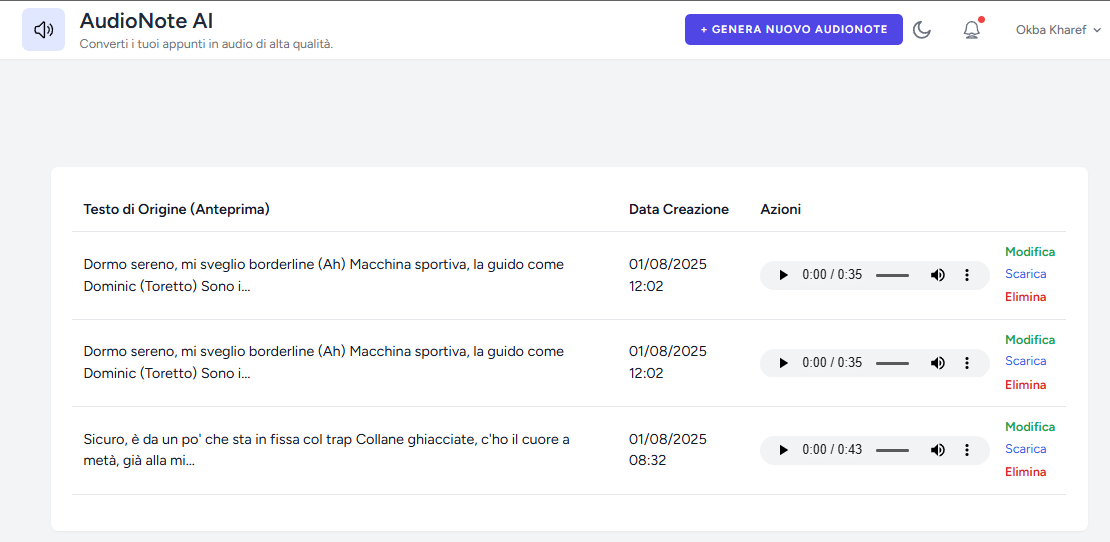
\includegraphics[width=6.5cm]{Screenshots/foglio3/problema83.png}\hspace*{\fill}
    \vspace{10pt}
    \\
    \hline
    \textbf{Nome del valutatore} & Kharef \\
    \hline
  \end{tabular}
\end{table}

% Problema \getNumeroProblema (Basato su Kharef P27)
\begin{table}[htbp]
  \centering
  \renewcommand{\arraystretch}{1.5}
  \begin{tabular}{|>{\raggedright\arraybackslash}p{7.5cm}|>{\raggedright\arraybackslash}p{7.5cm}|}
    \hline
    \rowcolor{green!30}
    \multicolumn{2}{|c|}{\textbf{Problema \getNumeroProblema}} \\
    \hline
    \textbf{Descrizione} & I contenuti generati dagli strumenti AI (trascrizioni e AudioNote) sono presentati come output "finali" e non modificabili. \\
    \hline
    \textbf{Pagina del sito} & Sbobinatore AI / AudioNote AI \\
    \hline
    \textbf{Principi violati} & 3 (Controllo e libertà dell'utente); 9 (Permettere all’utente di correggere gli errori e non solo di rilevarli) \\
    \hline
    \textbf{Grado di severità} & 2 (Problema secondario) \\
    \hline
    \textbf{Screen} &
    \vspace{10pt}
    \hspace*{\fill}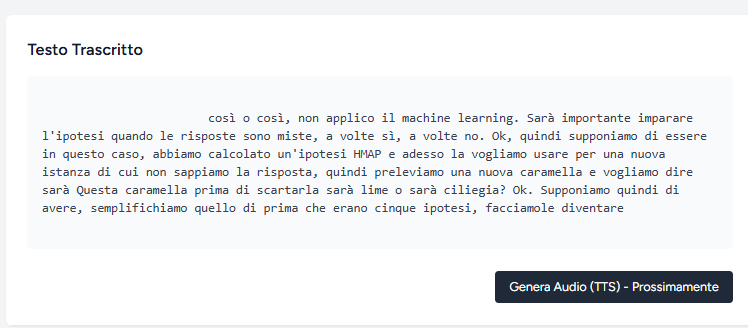
\includegraphics[width=6.5cm]{Screenshots/foglio3/problema85.png}\hspace*{\fill}
    \vspace{10pt}
    \\
    \hline
    \textbf{Nome del valutatore} & Kharef \\
    \hline
  \end{tabular}
\end{table}

% Problema \getNumeroProblema (Basato su Kharef P29)
\begin{table}[htbp]
  \centering
  \renewcommand{\arraystretch}{1.5}
  \begin{tabular}{|>{\raggedright\arraybackslash}p{7.5cm}|>{\raggedright\arraybackslash}p{7.5cm}|}
    \hline
    \rowcolor{green!30}
    \multicolumn{2}{|c|}{\textbf{Problema \getNumeroProblema}} \\
    \hline
    \textbf{Descrizione} & Non è presente una chiara distinzione visiva tra le proprie risorse (appunti caricati dall'utente) e le risorse della community quando si naviga in "Esplora Appunti". \\
    \hline
    \textbf{Pagina del sito} & Esplora Appunti \\
    \hline
    \textbf{Principi violati} & 1 (Far vedere lo stato del sistema); 5 (Riconoscimento piuttosto che uso della memoria dell’utente); 7 (Visualizzare tutte e sole le informazioni necessarie) \\
    \hline
    \textbf{Grado di severità} & 1 (Problema accessorio) \\
    \hline
    \textbf{Screen} &
    \vspace{10pt}
    \hspace*{\fill}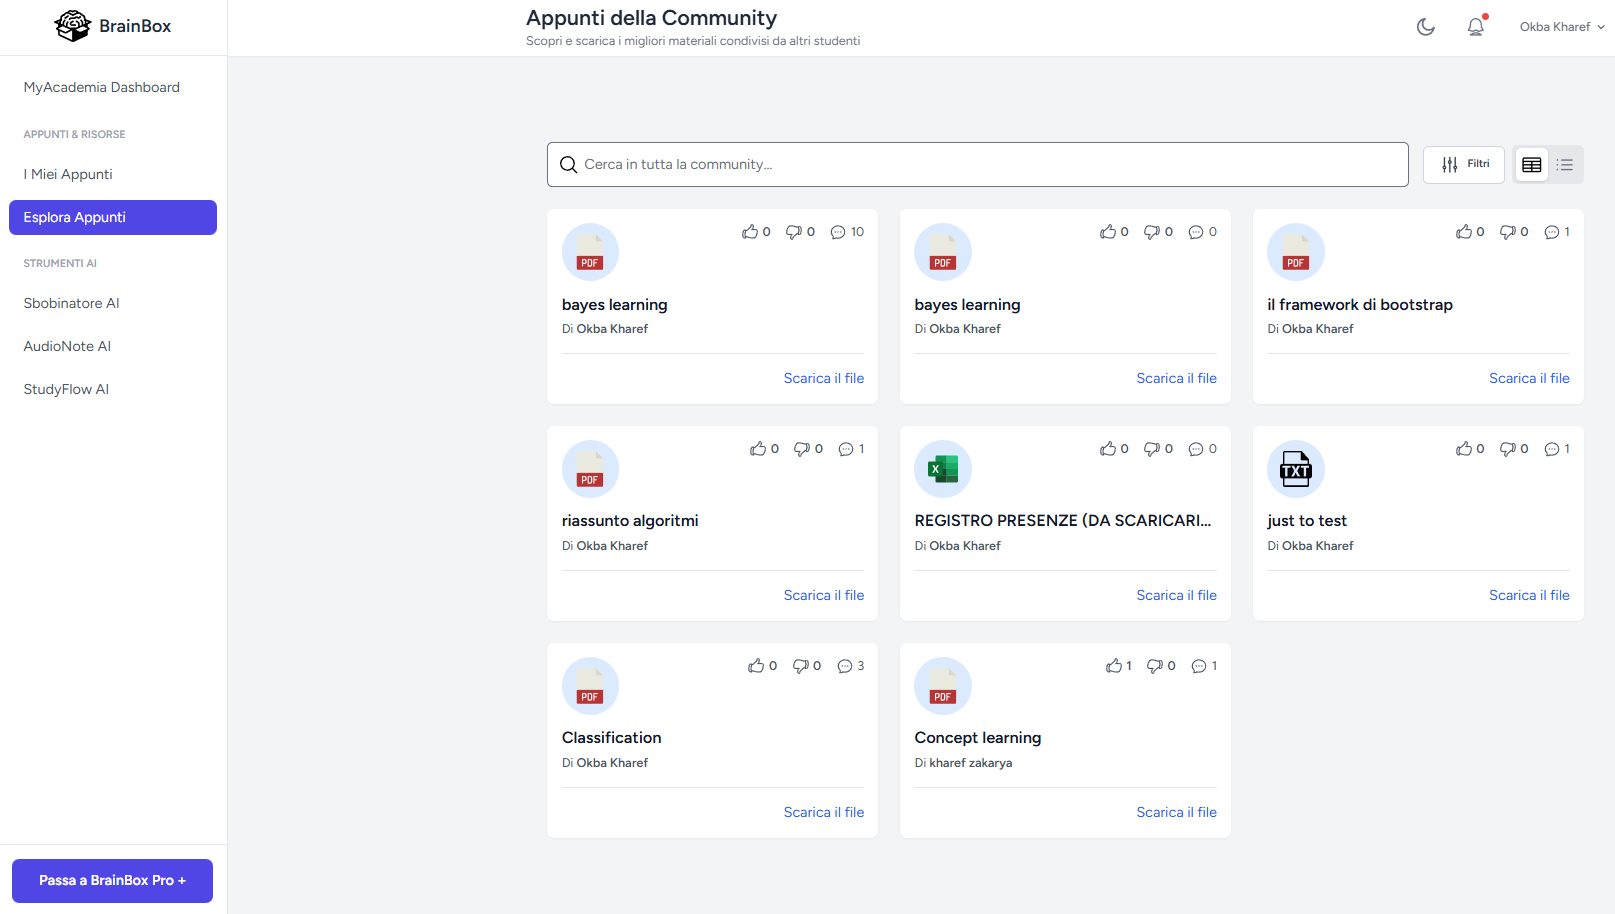
\includegraphics[width=6.5cm]{Screenshots/foglio3/problema74.png}\hspace*{\fill}
    \vspace{10pt}
    \\
    \hline
    \textbf{Nome del valutatore} & Kharef \\
    \hline
  \end{tabular}
\end{table}

% Problema \getNumeroProblema (Basato su Kharef P30)
\begin{table}[htbp]
  \centering
  \renewcommand{\arraystretch}{1.5}
  \begin{tabular}{|>{\raggedright\arraybackslash}p{7.5cm}|>{\raggedright\arraybackslash}p{7.5cm}|}
    \hline
    \rowcolor{green!30}
    \multicolumn{2}{|c|}{\textbf{Problema \getNumeroProblema}} \\
    \hline
    \textbf{Descrizione} & Le funzionalità basate su AI (Sbobinatore e Generatore AudioNote) non spiegano i loro limiti tecnologici (es. la qualità dipende dall'audio, la voce generata è sintetica), creando aspettative irrealistiche. \\
    \hline
    \textbf{Pagina del sito} & Sbobinatore AI / AudioNote AI  \\
    \hline
    \textbf{Principi violati} & 1 (Far vedere lo stato del sistema); 10 (Help e documentazione) \\
    \hline
    \textbf{Grado di severità} & 2 (Problema secondario)  \\
    \hline
    \textbf{Nome del valutatore} & Kharef \\
    \hline
  \end{tabular}
\end{table}

% Problema \getNumeroProblema (Basato su Kharef P32)
\begin{table}[htbp]
  \centering
  \renewcommand{\arraystretch}{1.5}
  \begin{tabular}{|>{\raggedright\arraybackslash}p{7.5cm}|>{\raggedright\arraybackslash}p{7.5cm}|}
    \hline
    \rowcolor{green!30}
    \multicolumn{2}{|c|}{\textbf{Problema \getNumeroProblema}} \\
    \hline
    \textbf{Descrizione} & I testi inseriti dagli utenti (descrizione degli appunti o commenti) non supportano alcuna formattazione di base (grassetto, corsivo, elenchi). Questo porta alla creazione di "muri di testo" poco leggibili. \\
    \hline
    \textbf{Pagina del sito} & I Miei Appunti \\
    \hline
    \textbf{Principi violati} & 6 (Assicurare flessibilità ed efficienza d’uso); 7 (Visualizzare tutte e sole le informazioni necessarie) \\
    \hline
    \textbf{Grado di severità} & 1 (Problema accessorio) \\
    \hline
    \textbf{Screen} &
    \vspace{10pt}
    \hspace*{\fill}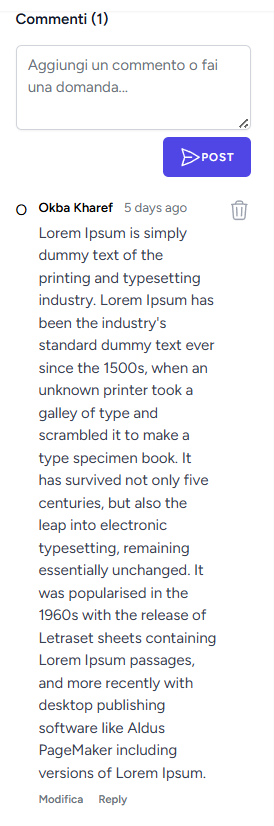
\includegraphics[height=6cm, keepaspectratio]{Screenshots/foglio3/problema90.png}\hspace*{\fill}
    \vspace{10pt}
    \\
    \hline
    \textbf{Nome del valutatore} & Kharef \\
    \hline
  \end{tabular}
\end{table}
